
\begin{figure*}[htbp]
  \centering
  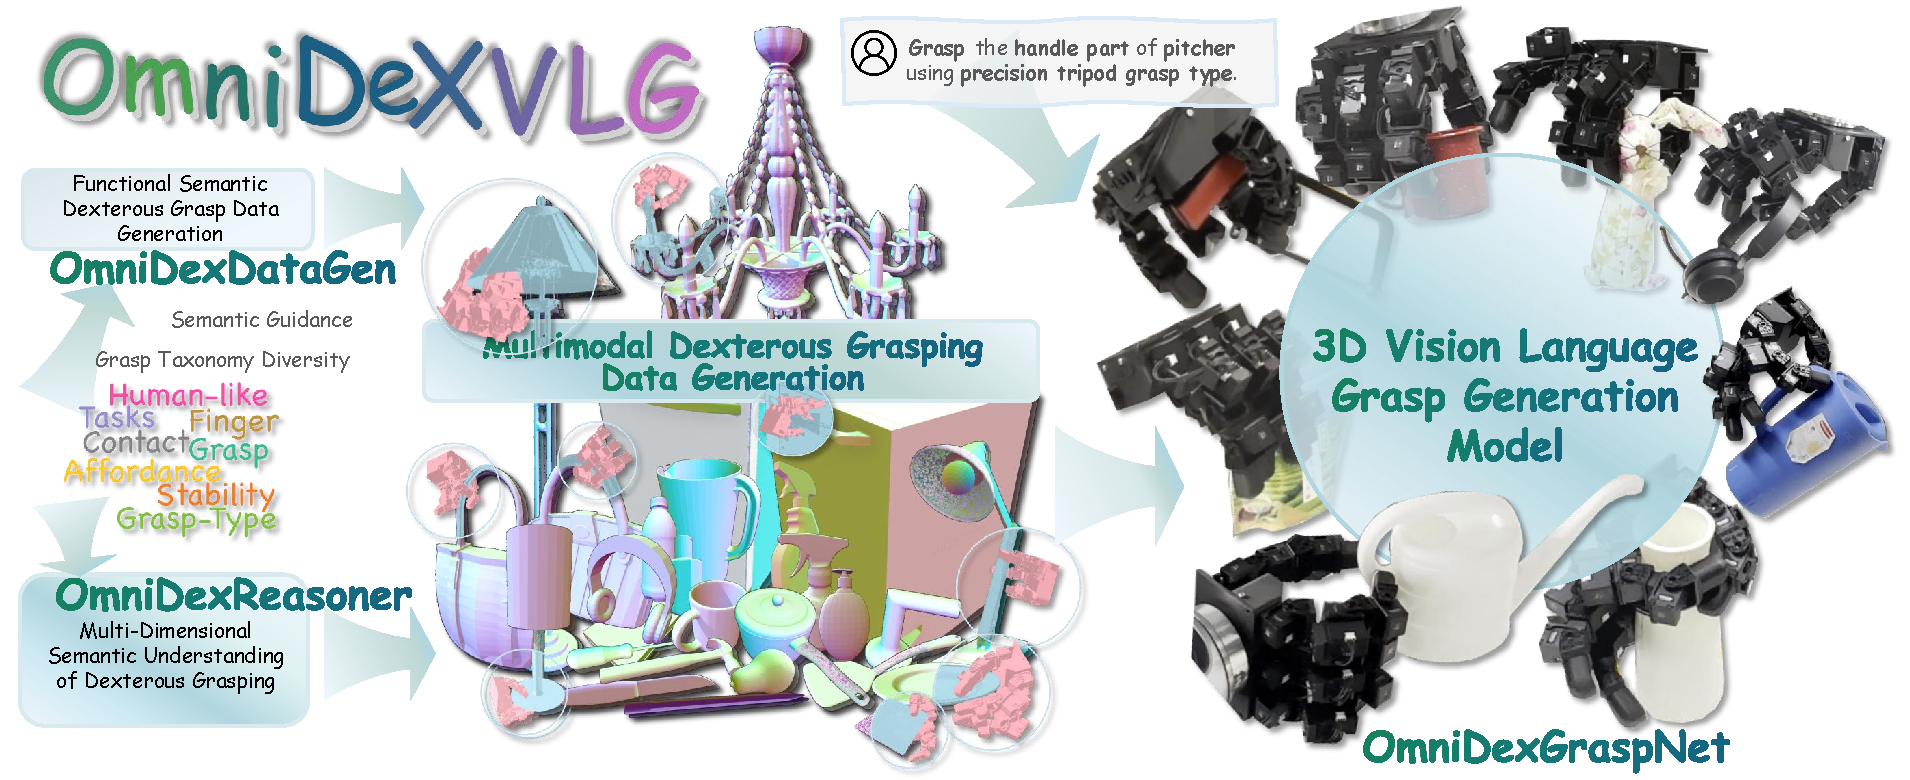
\includegraphics[width=1.0\linewidth]{pictures/fig0_heading_photo_ffh.pdf}
  \caption{%
  Overview of the OmniDexVLG framework. The framework integrates three core components: OmniDex-DataGen, for functional and grasp taxonomy-aware dexterous grasp dataset generation; OmniDexReasoner, for multi-dimensional semantic understanding using large multimodal models; and OmniDexGraspNet, a 3D vision-language grasp generation model guided by semantic instructions across grasp type, affordance, contact, and finger configuration. }
  \label{fig:heading_photo}
\end{figure*}
Dexterous hands, owing to their high degrees of freedom and complex manipulation capabilities, have demonstrated remarkable potential in fine-grained grasping and coordinated multi-finger tasks. In recent years, advancements in generative models and reinforcement learning have enabled researchers to synthesize reliable dexterous grasp poses from visual observations of objects, substantially improving grasp robustness and generalization across diverse objects and environments~\cite{wang2022dexgraspnet,murali2025graspgen}.

In real-world scenarios, dexterous hands are often required to perform grasping and manipulation tasks with multi-dimensional semantic intent. For example, a task might involve grasping the handle of a kettle using a tripod grasp with the thumb, index, and middle fingers. For humans, such semantic reasoning is naturally achievable through prior knowledge and experience. To model this reasoning process, the concept of grasp taxonomy~\cite{feix2015grasp} has emerged as a structured framework that categorizes grasp strategies based on finger, contact point configurations, opposition types, and force directions, thereby formalizing the diversity of grasp behaviors in both human and robotic hands.

However, existing semantic-guided grasp generation approaches primarily focus on functional grasping, lacking explicit sensitivity to grasp taxonomy and contact semantics~\cite{tang2023graspgpt,tang2025foundationgrasp,li2024semgrasp,huang2025fungrasp,agarwal2023dexterous}. In the context of objects with multiple functional affordance regions, different task goals often require distinct grasp strategies beyond the simplistic alignment with functional parts. Critical semantic elements such as finger flexion, contact configurations, and force application are highly correlated with the intended grasp type, yet current models struggle to utilize such fine-grained cues, resulting in limited controllability and semantic diversity in generated grasp actions.

Most existing dexterous grasp datasets~\cite{wang2022dexgraspnet,zhang2024contactdexnet} are constructed through optimization-based methods that guide hand-object distances while satisfying quality metrics like differential force closure (DFC)~\cite{liu2021synthesizing}. While some recent works have introduced multimodal conditioning to enhance semantic grounding, these models largely focus on part-level semantics or predefined functional goals. They lack the capacity to model and generalize structured grasp semantics, including contact semantics, grasp taxonomy, and affordance-sensitive representations~\cite{wang2022dexgraspnet,zhang2024contactdexnet,murali2025graspgen,zhong2025dexgrasp}. This leads to sparse distributions of grasp types in existing datasets~\cite{wang2022dexgraspnet,zhong2025dexgrasp}. For instance, datasets like DexGraspNet~\cite{wang2022dexgraspnet} are dominated by simplified grasp types such as the pinch grasp, exposing the limitations of current models in generating diverse contact structures and grasp configurations. Although some studies have introduced manually annotated grasp-type labels~\cite{chen2025dexonomy}, how to automatically generate diverse and semantically meaningful grasp types remains an open challenge. 

To address these limitations, we propose a novel grasp data generation framework (OmniDexDataGen) that integrates functional affordance cues, contact pattern priors, and finger configuration semantics. This enables the synthesis of grasp samples that are not only physically stable, but also semantically rich and structurally diverse—providing stronger priors for downstream reasoning and generation tasks.

Furthermore, even in existing datasets with semantic labels, the grasp-related semantics are often coarse and limited to object-level part annotations~\cite{song2025learning} or basic functional descriptors~\cite{zhang2023functionalgrasp}. There remains a lack of a unified semantic understanding model capable of jointly reasoning about grasp taxonomy, contact semantics, and functional affordance. Given the inherent complexity of dexterous hands, semantic reasoning in this context requires modeling the nuanced relationships between hand-object contact topology, force dynamics, and task-driven semantic objectives. The object’s affordance often constrains which grasp types are viable and, in turn, influences the contact structure and pose planning strategy required for successful manipulation. 

Motivated by these challenges, we introduce a multimodal semantic understanding framework based on large multimodal models (LMMs), named OmniDexReasoner, tailored for reasoning over dexterous grasping tasks. Our framework seeks to unify the modeling of grasp type, contact structure, and functional intent under a shared semantic space, enabling fine-grained understanding and generation of natural language grasp instructions for dexterous hands.


To further bridge the semantic gaps in current grasp generation pipelines, especially in representing grasp taxonomy, contact semantics, and affordance, we propose a vision-language grasp generation (VLG) model, OmniDexGraspNet, for semantically grounded grasp generation. By combining multimodal inputs, including language instructions and visual point clouds, with multi-dimensional semantic modeling, our method enables joint reasoning over complex task goals and grasp semantics. This facilitates the generation of grasp poses that are both semantically aligned and physically plausible. Through explicit modeling of structured semantics and controllable generation, our approach not only improves the diversity and realism of generated grasps, but also lays a foundation for more generalized, task-aware robotic manipulation.

Our Contributions are summarized as follows:
\begin{itemize}
\item \textbf{OmniDexDataGen: Functionality-Aware and Contact-Sensitive Dexterous Grasp Dataset Generation Method with Grasp Taxonomy Diversity.} We propose an optimization-based framework for generating dexterous grasp datasets that are sensitive to grasp taxonomy, hand-object contact points, and functional affordance. 
Our approach substantially enhances the dataset's representational richness in terms of contact guidance and grasp semantics. Furthermore, it improves the diversity of grasp types, contact paradigms, and functional affordances.

\item \textbf{OmniDexReasoner: LMM-Based Functional, Contact, and Taxonomy-Aware Dexterous Grasp Understanding Method.} 
We propose an LMM-powered framework for dexterous grasping that captures multi-level semantic cues across three core dimensions: functional affordance, contact semantics, and grasp taxonomy. By incorporating a multi-agent collaboration mechanism, retrieval-augmented generation (RAG) and Chain-of-Thought (CoT) reasoning, the proposed method addresses key limitations in current multimodal understanding approaches for dexterous hands, substantially enhancing the comprehension of complex grasping behaviors. 

\item \textbf{OmniDexGraspNet: Semantic-Aware 3D Vision-Language Grasp Pose Generation Model.} 
We propose a grasp pose generation method that integrates a 3D vision-language model to guide dexterous grasp synthesis using multi-dimensional semantic information and partial object point clouds. The method enables the generation of grasp poses that are sensitive to various semantic dimensions, including functional intent, grasp taxonomy, and contact configuration. It demonstrates strong generalization across objects of different sizes and categories, producing diverse functional grasps with rich semantic and structural variability. Compared to existing grasp generation approaches, our method exhibits superior semantic sensitivity and grasp diversity.

\end{itemize}


